%\title{Using the forest package to create trees in LaTeX}
% From http://tex.stackexchange.com/a/108728/23931 
\documentclass[12pt,preview,border=0]{standalone}
\usepackage[paperheight=6cm,paperwidth=15cm]{geometry}
\usepackage{graphicx}
% \usepackage{forest}
\usepackage{amsmath}
% \usepackage{txfonts}  %pretty math font
\usepackage{kmath,kerkis}
\usepackage{tikz}
\usetikzlibrary{arrows,automata,positioning}

% fontspec requires xelatex/lualatex
% \usepackage{fontspec}
% \setmainfont[Scale=1,Ligatures={Common}]{Adobe Caslon Pro}
% \setromanfont[Scale=1,Ligatures={Common}]{Adobe Caslon Pro}

%%%%%% XeLaTeX Math Font Setup #%%%%%%%%%%%%%%
% \usepackage{bm}
% \usepackage{mathspec}
% \usepackage{xltxtra}  % also loads fontspec
% \usepackage{xunicode}
% \usepackage{fontspec}
% \defaultfontfeatures{Mapping=tex-text}
% \setmainfont[Scale=1,Ligatures={Common}]{Adobe Caslon Pro}
% \setromanfont[Scale=1,Ligatures={Common}]{Adobe Caslon Pro}
% \setmathrm[Scale=1]{Adobe Caslon Pro}
% \setmathfont(Digits,Latin)[Numbers={Lining,Proportional}]{Adobe Caslon Pro}
%%%%%%%%%%%%%%%%%%%%%%%%%%%%%%%%%%%%%%%%%%%%%%


%%%%%%%%%%%%%%%%%%%%%%%%%%%%%
% \usepackage{fontspec,mathfont}
% \setmainfont{Adobe Caslon Pro}
% % \setmathfont{Adobe Caslon Pro}
% \mathfont{Cambria Math}
%%%%%%%%%%%%%%%%%%%%%%%%%%%%%
\begin{document} 
\begin{center}
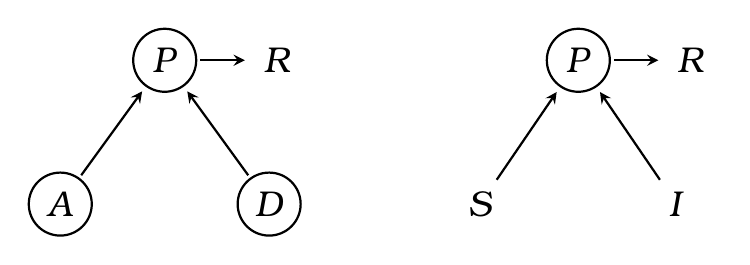
\begin{tikzpicture}[
	> = stealth, % arrow head style
	shorten > = 1pt, % don't touch arrow head to node
	auto,
	node distance = 2cm, % distance between nodes
	thick, % line style
	U/.style={circle, draw=black, inner sep=1.8pt, outer sep=1.5pt, minimum size=8mm, font=\Large},  %draw=black, fill=white
	O/.style={circle, inner sep=3.4pt, outer sep=-.75pt, minimum size=8mm, font=\Large},              %draw=white, fill=white
	]
	
	% Nodes and their relative positions
	\node[U] (P) [] {$P$};
	\node[O] (anc) [below =  1 of P] {};
	\node[U] (A)   [left  = .5 of anc] {$A$};
	\node[U] (D)   [right = .5 of anc] {$D$};
	\node[O] (R)   [right = .6 of P] {$R$};

	% Paths connecting nodes
	\path[->] (A) edge (P);
	\path[->] (D) edge (P);
	\path[->] (P) edge (R);


	% Nodes and their relative positions
	\node[U] (P2) [right = 3 of R] {$P$};
	\node[O] (anc2) [below =  1 of P2] {};
	\node[O] (S)   [left  = .5 of anc2] {$S$};
	\node[O] (I)   [right = .5 of anc2] {$I$};
	\node[O] (R2)   [right = .6 of P2] {$R$};

	% Paths connecting nodes
	\path[->] (S) edge (P2);
	\path[->] (I) edge (P2);
	\path[->] (P2) edge (R2);

\end{tikzpicture}
	

\end{center}\end{document}
